\section{Theorie}
\label{sec:Theorie}
Zur Messung ionisierender Strahlung wird das Geiger-Müller-Zählrohr genutzt, an dessen Ausgang kann ein
Impulszähler angeschlossen und damit kann die Intensität der Strahlung gemessen werden.
Die Apparatur besteht aus einem Metallzylinder, dieser dient als Kathode, und einem Anodendraht. Das Innere ist gefüllt mit einem Gasgemisch
aus Argon und Ethylalkohol.
Beim Anlegen einer Spannung entsteht ein elektrisches Feld, damit wird die Bewegung der eingehenden Teilchen beeinflusst.
Die Teilchen weisen unterschiedliches Verhalten bei verschiendenen Spannungen auf, somit enstehen verschiedene Abschnitte, wie
in Abbildung \ref{fig:bereich} zu sehen.
\begin{figure}
  \centering
  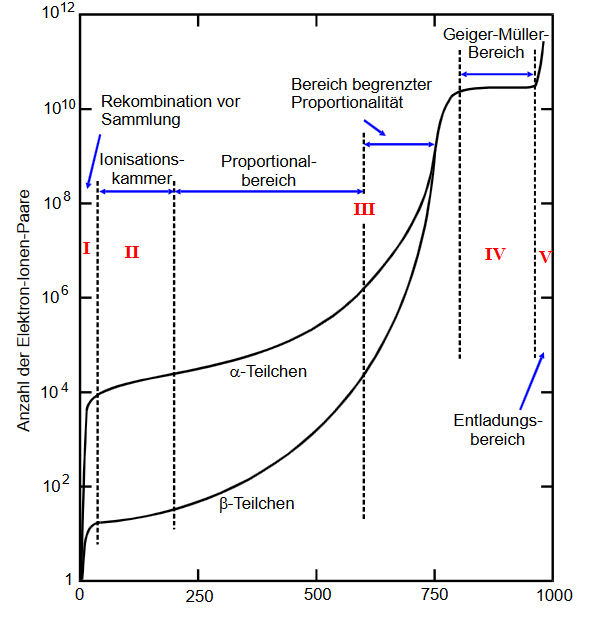
\includegraphics[width=0.4\textwidth]{bereiche.PNG}
  \caption{Verschiedene Zonen des Widerstandes.\cite{sample}}
  \label{fig:bereich}
\end{figure}
Zone $I$ stellt die geringen Spannungen dar, dabei erreichen kaum Elektronen den Draht, zuvor rekombinieren diese.
In Zone $II$ kommen wegen der höheren Spannung fast alle Elektronen bei der Anode an. Hier ist der Ionisationsstrom proportional
zur Energie der einfließenden Strahlung.
In Zone $III$ ist die Spannung so groß, dass die Elektronen genung Energie besitzen um selbst zu ionisieren. Es kommt zur Kettenreaktion
welche Townsend-Lawine genannt wird. Die Ladung $Q$ am Draht ist jetzt groß genug, dass Ladungsimpulse gemessen werden können.
In Zone $IV$ liegt der Auslöserbereich, der eigentliche Arbeitsbereich des Geiger-Müller-Zählrohrs. Hier ist $Q$ nicht mehr abhängig
von der Primärionisation. Hier entstehen auch UV-Photonen welche sich in Richtung des E-Feldes und senkrecht dazu ausbreiten,
damit breitet sich auch die Elektronenlawiene im gesammten Gasraum aus.\\
Ein Effekt der beim Geiger-Müller-Zahler auftritt ist der Ionenschlauch, die positiven Ionen bilden auf Grund ihrer Trägheit
einen Schlauch um den Anodendraht und damit auch ein Gegenfeld.
Durch diesen Effekt wird, in der sogenannten Totzeit, durch ionisierende Strahlung
keine Lawine ausgelöst. Nach der Totzeit folgt die Erholungszeit, dabei fallen die gemessenen Impulse schwächer aus. Dieser Sachverhalt ist in Abbildung
\ref{fig:totzeit} dargestellt.
\begin{figure}
  \centering
  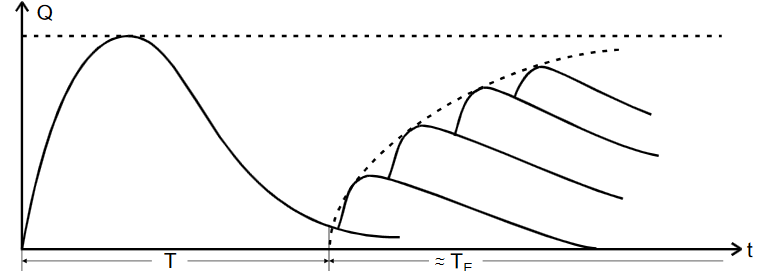
\includegraphics[width=0.6\textwidth]{tz.PNG}
  \caption{Totzeit und anschließende Erholungszeit im Q-t-Diagramm.}
  \label{fig:totzeit}
\end{figure}
Einen weiteren unerwünschten Effekt bilden die Nachentladungen. Ionen sind in der Lage Elektronen aus der Metallwand rauszuschlagen,
diese Elektronen tragen zu den registrierten Impulsen bei. Mit Alkoholdämpfen können die Nachentladungen reduzierte werden, die
Ionen geben dann Energie an die Langen Alkoholmolekühle ab.\\
Von Interessse ist auch die Charakteristik des Zählrohrs. Diese entspricht der registrierten Teilchenzahl $N$ in Abhängigkeit von der
angelegten Spannung bei konstanter Strahlungsintensität. Eine Charakteristik hat etwa die Gestalt wie in Abbildung \ref{fig:char}.
\begin{figure}
  \centering
  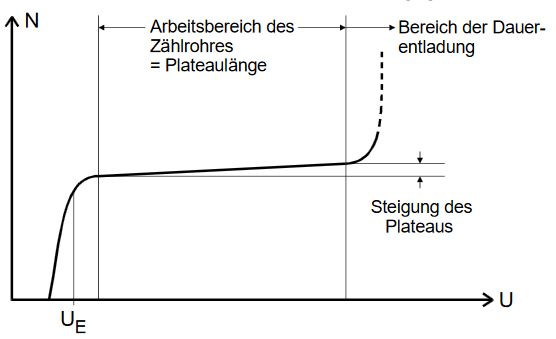
\includegraphics[width=0.6\textwidth]{char.PNG}
  \caption{Charakteristik eines Zahlrohres.}
  \label{fig:char}
\end{figure}
Das Plateau sollte idealerweise eben sein, dies ist auf Grund der Nachentladungen meist nicht der Fall.
Bei Spannungen außerhalb des Arbeitsbereiches kommst es zur selbstständigen Gasentladungen und damit zur Zerstörung des Zählrrohres.
\newpage
